% Chapter Template

\chapter{Implementation} % Main chapter title

\label{Chapter5} % Change X to a consecutive number; for referencing this chapter elsewhere, use \ref{ChapterX}

%----------------------------------------------------------------------------------------
%	SECTION 1
%----------------------------------------------------------------------------------------

\section{Data collection and cleaning}

The key foundation of the project was being able to collect the data that would allow the creation of the well-being domain scores. Collecting the required data and shaping it into the formats that were needed was, in places, one of the most challenging aspects of the project and the one that required the largest proportion of time. This part of the project presented several challenges that needed to be overcome.

%-----------------------------------
%	SUBSECTION 1
%-----------------------------------
\subsection{Collection of data files}

For ward level data, the Greater London Authority's datastore is a primary data source. A significant proportion of the data for the creating of the well-being indicators could be accessed via this source. 

%-----------------------------------
%	SUBSECTION 2
%-----------------------------------

\subsection{Collection from APIs}

The API that was key to the success of the project was that of social media platform Foursquare. To represent community vitality, the aim was to create a measure for the restaurants and bars in each ward. Foursquare is a platform based around venue information so holds the information required for this measure. Foursquare also holds information on cultural venues. Therefore the measure of 'Access to Cultural Space' could also be obtained from this platform.
To use the API to obtain venue information you are required to search for venues within a specified radius of a certain point, given in latitude and longditude. The challenge with Foursquare was the the API rate limits which limits each search to a maximum of 49 searches. There are also daily and monthly rate limits to stay within.
To obtain results of all bars, restaurants and cultural venues accross Greater London with these limits an iterative algorithm had to be created which could travel accross London by latitude and longditude, taking in small enough areas so as to not exceed 49 results a time. To achieve this, I created a latitude and longditude bounding box around London and created a nested loop iteration of 50 points of latitude and 50 points of longditude. The areas created by this had some overlap so as not to have missing areas of the capital. With a counter to check if the search limit of 49 venues was exceeded, this search algorithm put the list of venues into a pandas dataframe and de-duplicated for where areas had ovelapped.

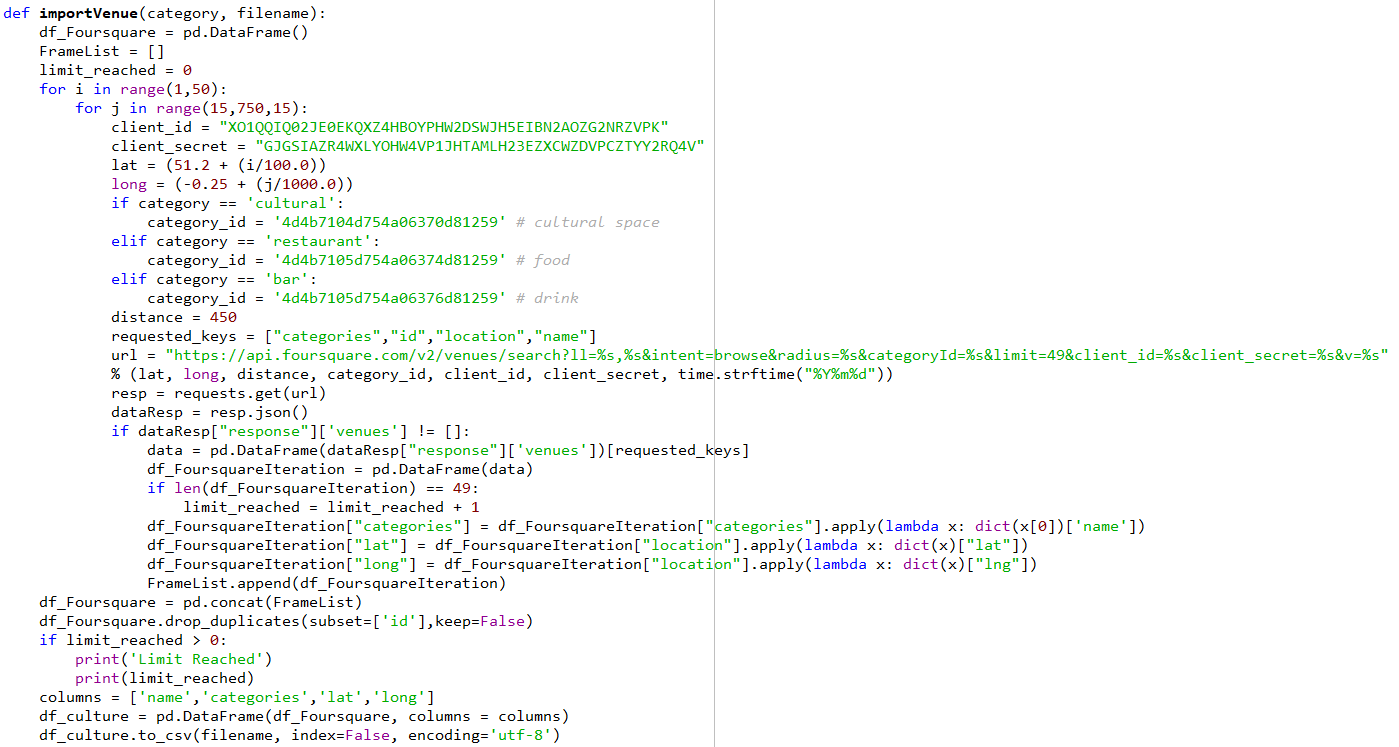
\includegraphics[scale=0.75]{figures/API_import} % Code example

Because of the rate limits, running the algorithm for such a large area could only be done on a daily basis.

%----------------------------------------------------------------------------------------
%	SECTION 2
%----------------------------------------------------------------------------------------

\section{Well-being domain scores}

The motivation for creating composite domain scores 6 different measures of well-being was two-fold. Firstly creating a score for each domain over a pre-defined scale would allow users of the front-end interactive map compare scores accross wards and give those scores some contextual meaning and significance. With 6 domains rather than the original 18 datasets, the amount of information presented to the user would not be too large to prevent a non-technical audience from interpreting the information on the map. The second reason for creating the domain indicators was to help to try and create an interpretable model rather than one requiring significant dimension reduction. Whilst some less interpretable models will be tested to validate the quality of the quintile classification model, ideally the project and the user front end should allow us to draw some conclusions about any link between well-being and median house prices in London.

For each domain three appropriate datasets were chosen and then reduced to give a single score for each ward. The 3 datasets for each domain were standardised using a function in Python and those which related to a negative indicator such as emissions or crime were mutliplied by a value of -1. Using this technique of standardisation gave equal weighting to each of the three indicators. Because of the equal weighting given to each indicator, these can be seen as substitutable within the context of the domain which is a important factor in the choice of technique used to reduce the indicators to a score. With indicators that can be assumed to be substitutable suitable techniques would include Principal Component Analysis (PCA) and an arithmetic mean
?INSERT REFERENCE TO PAPER BY ITALIAN ACADEMICS?
For the 6 domains, a mixture of the two techniques have been used. For those domains where the 3 indicators have a relatively high correlation ?ABOVE WHAT? the first Principal Component has been used to try and extract the largest amount of variance within the three indicators. Where the indicators for a domain have low levels of correlation for at least one of the three datasets, the arithmetic mean has been used. This approach gives us three domains which use PCA and three which use the mean.
?INSERT COV MATRICES AND TECHNIQUES FOR EACH DOMAIN?
This approach tries to maximise the information contained in all of the datasets.
To create an interpretable and comparable score for each domain the resulting single scores have been normalised and then rescaled to be between 0 and 100, this is the score that is presented in the user front end.


%----------------------------------------------------------------------------------------
%	SECTION 3
%----------------------------------------------------------------------------------------

\section{London house prices as a regression problem}

London is known for having very high real estate values but we can see from the map below that there are specific wards, particularly in the western central area, where median house prices are significantly above the Greater London area as a whole.

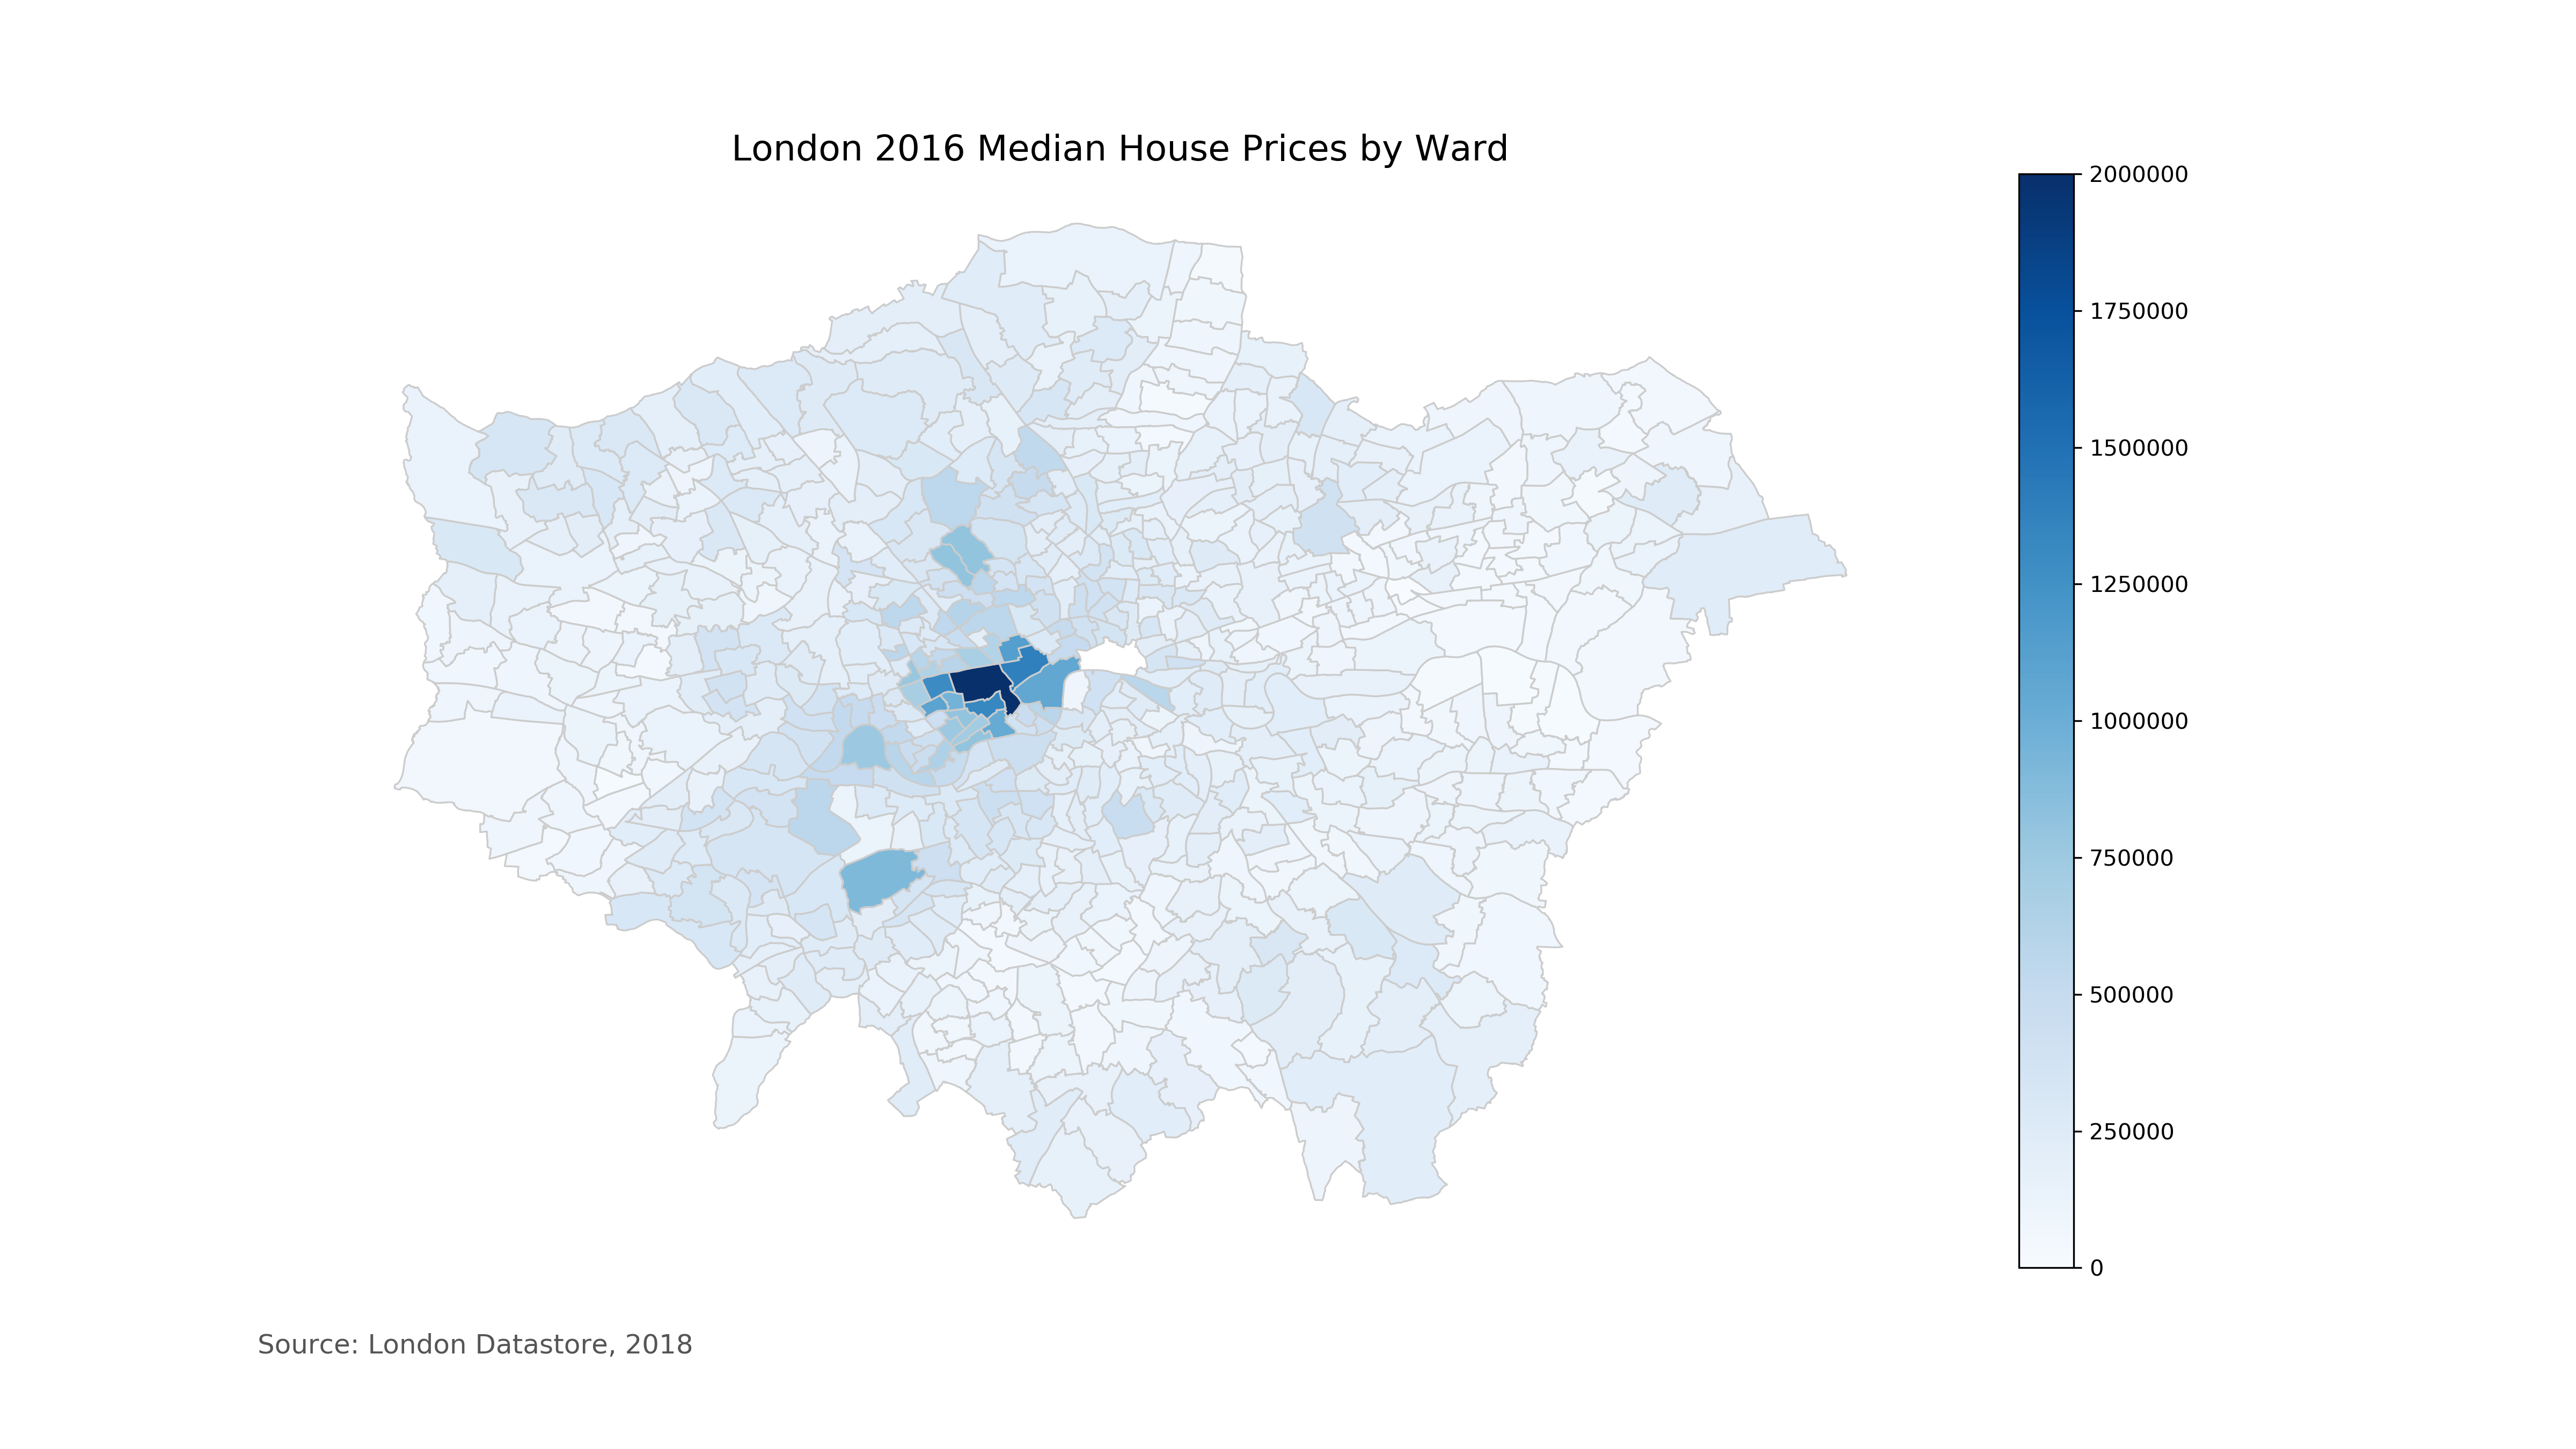
\includegraphics[scale=0.4]{figures/HPMedian} % Choropleth of median house prices

The choropleth map would suggest a high number of wards fall at the lower end of the range of median house prices with a small number with significantly high prices. From the pairwise plot below, the shape of the histogram of median house prices by ward would suggest that a power law may best describe the distribution.

? FIT POWERLAW TO MEDIAN HOUSE PRICES ?

For the domain scores, the histograms show most of the six as being at least close to a normal distribution. This is less clear in the case of the Safety and Security and Community Vitality and Participation domains with Safety and Security showing a large number of high values and Community Vitality and Participation showing many low scores. This can be attributed to a small number of wards where crime is high and that wards in central London have much greater access to both cultural and social spaces as indicated on the maps below. In both cases, a power law may best describe these distributions.

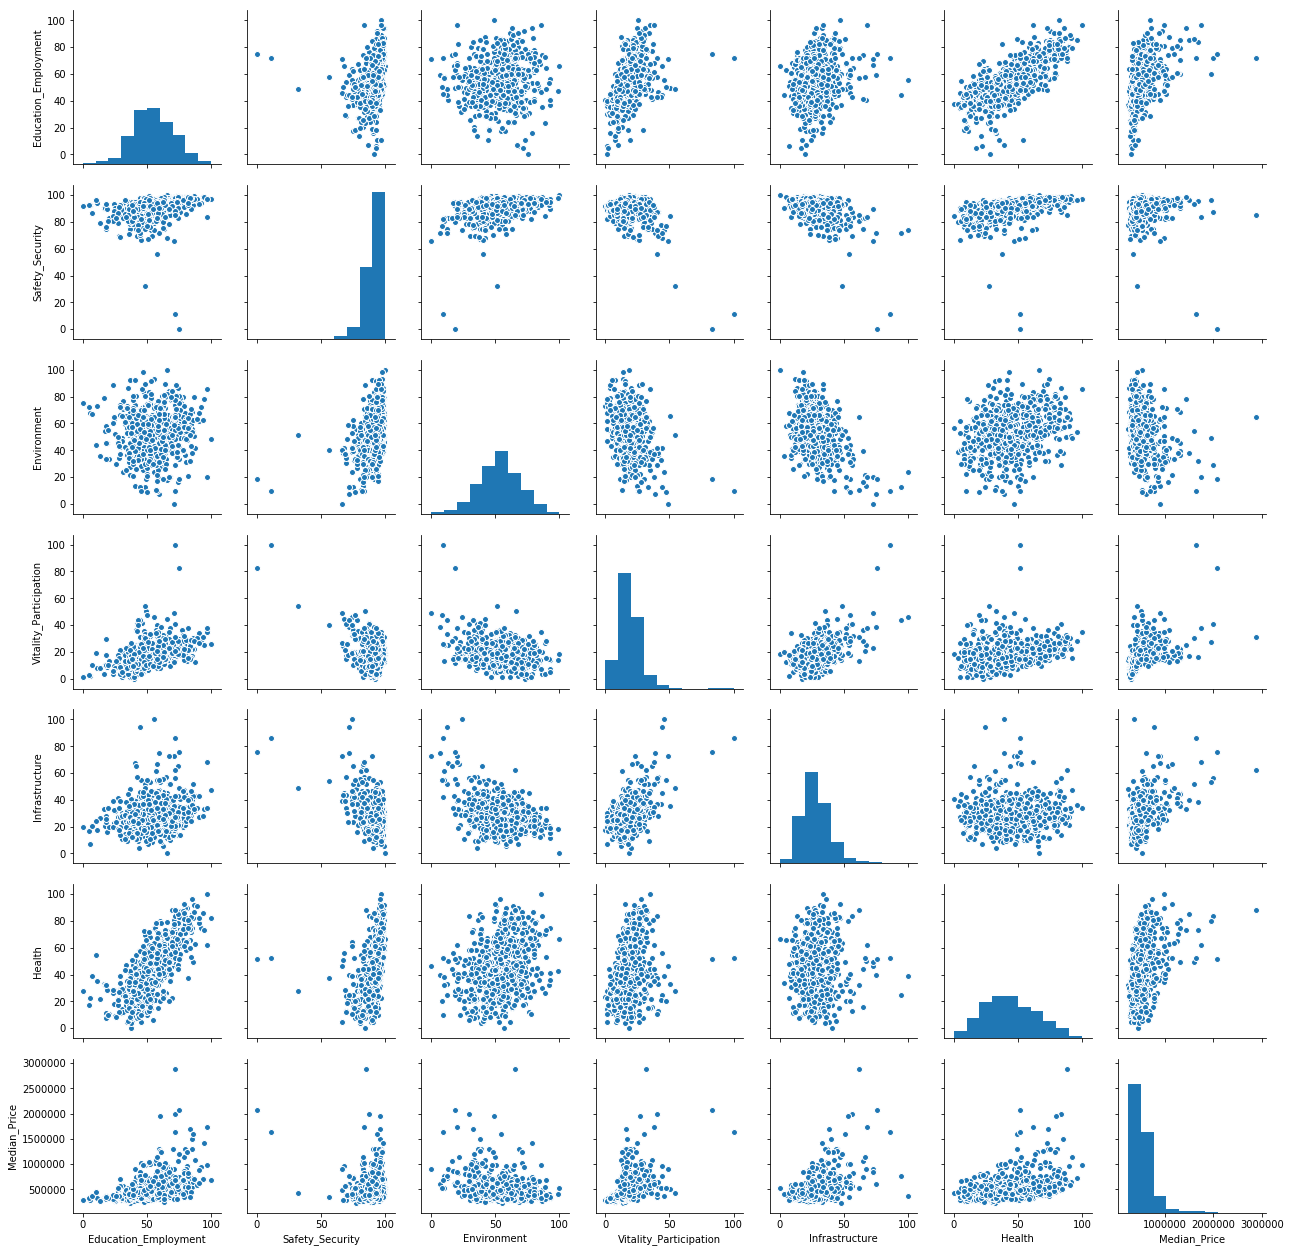
\includegraphics[scale=0.3]{figures/pairplot} % Pair-wise plot with median prices

This is less clear in the case of the Safety and Security and Community Vitality and Participation domains with Safety and Security showing a large number of high values and Community Vitality and Participation showing many low scores. This can be attributed to a small number of wards where crime is high and that wards in central London have much greater access to both cultural and social spaces as indicated on the maps below. In both cases, a power law may best describe these distributions.

Correlations

?INSERT MAPS OF EACH DOMAIN?

To begin the task of trying to model the median house prices from the well-being indicators, a simple multiple linear regression model was used with all six domains as predictors. The results show that this model explains less than half the variance with an R sq score of 0.39. There is enough to suggest that some form of linear model may provide a reasonable model of this problem.
To validate the model K-fold cross validation was used with k=7 with accuracy scores and mean squared errors average accross the seven iterations.

? STATSMODEL ?

Next a polynomial model was tried with degree two. This model explained almost none of the variance with an R sq value of very close to 0. The mean squared error also increased dramatically. The polynomial model does not seem to be a strong candidate for solving the problem.

The next models involved some feature reduction based on the p values of the domains in the original linear model. This meant that first Education and Employment were removed and then Community Vitality and Participation. This resulted in a small improvement in the model fit but little improvement in the MSE. 

With the median house price distribution suggesting a power law, a log transformation was performed on the data to try and linearise it with the linear regression model then re-run. This transformation dramatically increased the R sq value of the model, to 0.64, an increase of 0.25 from the equivalent model without the transformation. The model run on the log transformed data explains an additional 25 percent of the variance within the model. The exponent of the MSE is also a substantial reduction. This returned the following model:

?[insert model equation]?

As the best performing regression model this will be used for prediction in the final visulisation.

When the predictions were given the inverse transformation and validated against the actual values, the majority of wards showed that this model had good predictive capability although there were a handful of wards where the prediction had a signifcant error margin. The wards with significant errors tended to be those which had a much higher or lower score in a particular domain as compared to the neighbouring areas.

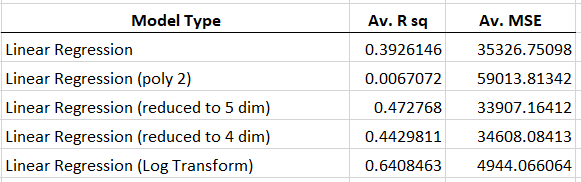
\includegraphics[scale=1]{figures/regression_results} % Regression results


%----------------------------------------------------------------------------------------
%	SECTION 4
%----------------------------------------------------------------------------------------

\section{London house prices as a classification problem}

The choropleth map below shows a different picture of London house prices being based on quintiles rather than monetary values, here the fifth quintile covers a larger range of values than the other quintiles due to the extremely expensive areas such as Knightsbridge and Belgravia where the median house price reaches over £2.8 million, 10 times as much as North End ward in Bexley.

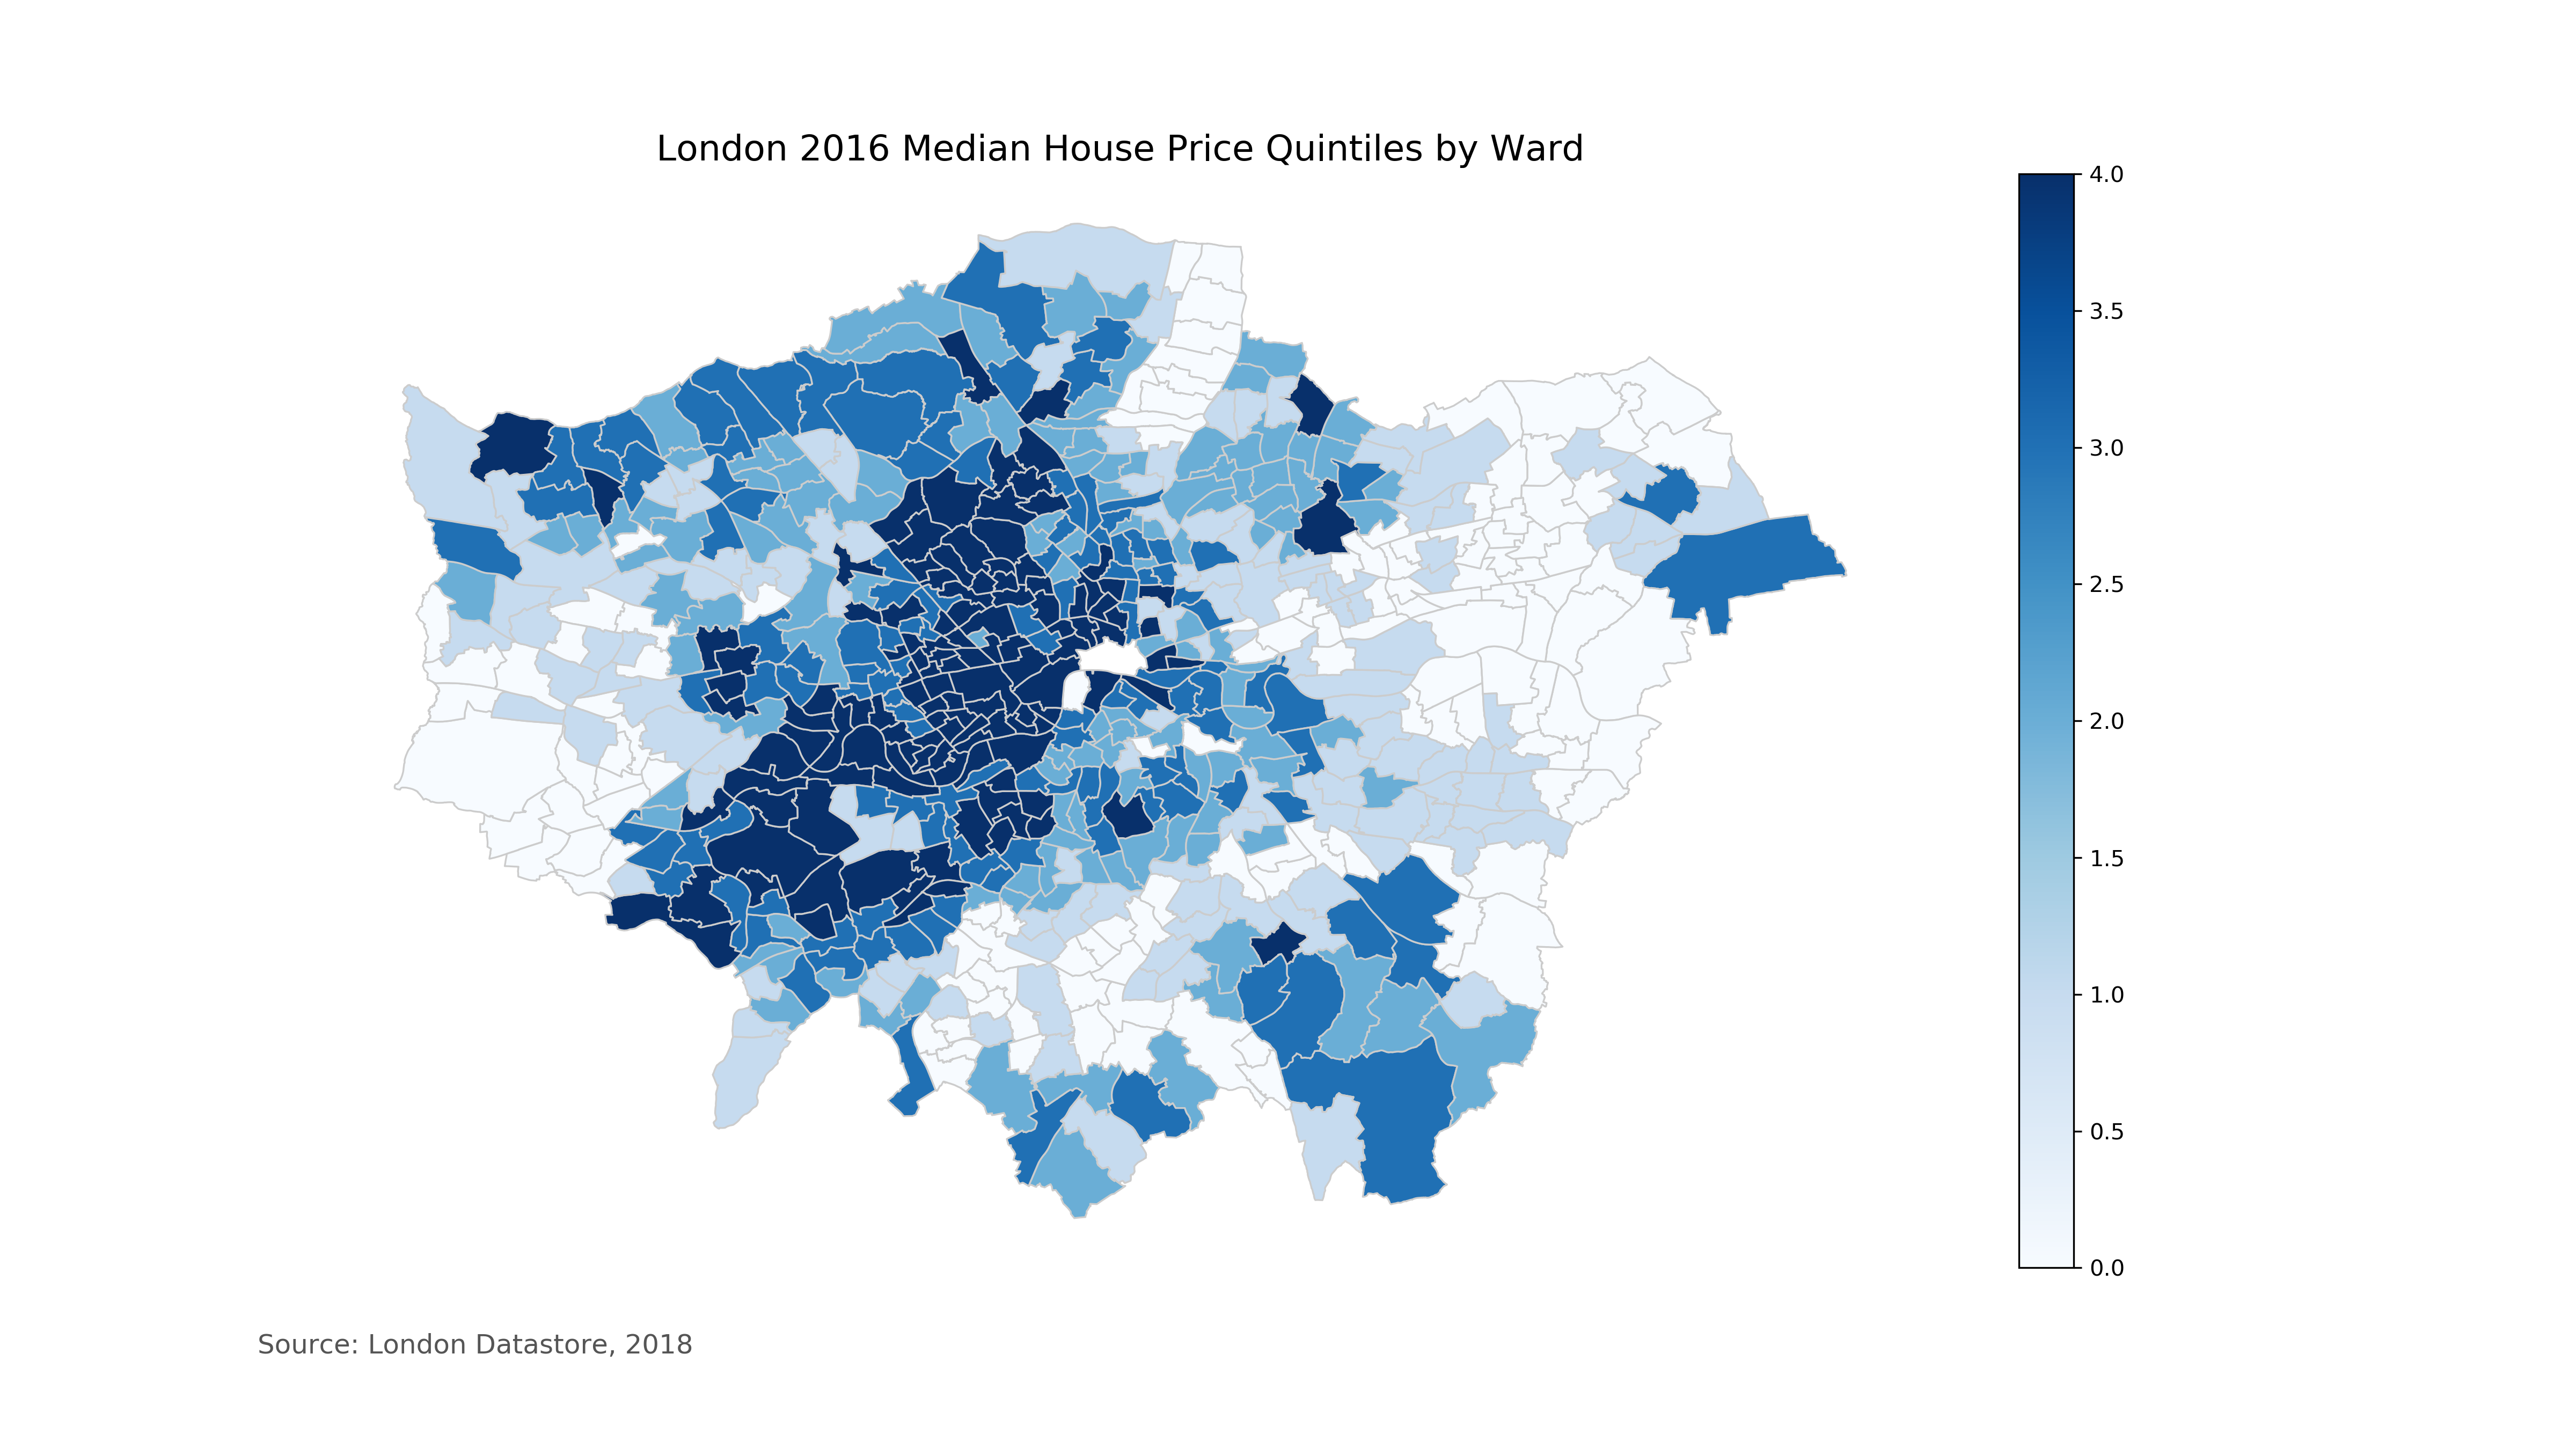
\includegraphics[scale=0.4]{figures/HPQuintile} % Choropleth of Median house prices by quintile

? BOXPLOT WITH QUINTILES ?

For the classification problem the aim was to try to find a model that has both a good fit and high interpretability. However, models that often have high accuracy but low interpretability such as support vector machines and neural networks were also used to both discover and validate the best classification model for the problem.

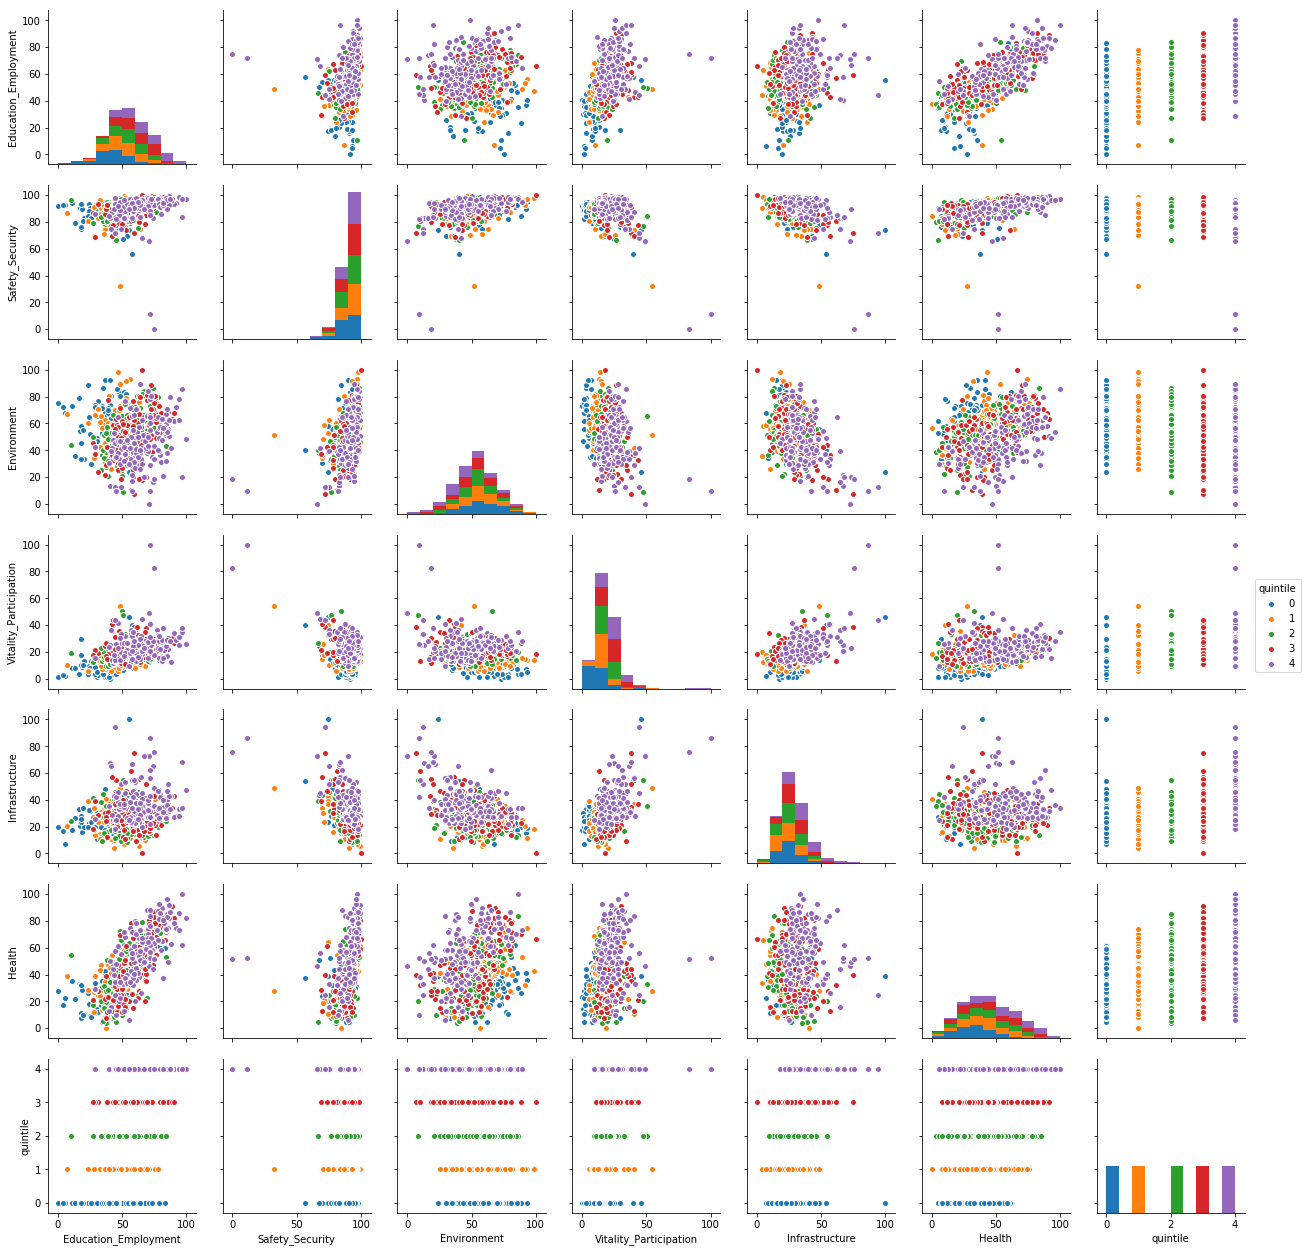
\includegraphics[scale=0.3]{figures/pairplot_quintile} % Pair-wise plot with median prices by quintile

By using the pair-wise plot and colouring the points by quintile, it is clear that there is no clear separation of quintile for any of the indicators with a more gradual movement from first to fifth quintile for most domains. Environment and Saftey and Security have an almost inverse relationship with the quintiles. Because the majority of the high-priced wards are centrally located, this may relate to a lack of greenspace and higher polution centrally as well as providing high-value targets for crime. 

? FINISH WRITING UP CLASSIFICATION MODELLING ?


%----------------------------------------------------------------------------------------
%	SECTION 5
%----------------------------------------------------------------------------------------

\section{Encoding as geoJSON}

To use the information from the creation of the well-being domains and the predictions obtained from the models in a javascript based visualisation, the information needed to be converted from a pandas dataframe in Python to a geoJSON file in javascript. A geoJSON file is a variation on the JSON format as defined below:

? GEOJSON DEFINITION ?

Whilst a relatively straightforward task within the geopandas module in Python, geoJSON accepts coordinates in latitude and longditude and the shapefile being used has the coordinates defining the ward polygons in Ordnance Survey grid references. To change this to latitude and longditude required the creation of a function that would take each polygon in the ward geometry in the geo data frame and break this down into the individual points which define the polygon. Once separated into coordinate pairs, these pairs could be reprojected to be latitude and longditude. The function was then required to recombine all of the coordinate pairs into the correct polygon geometries.

? CODE SNIPPET?

The information was then in the required format to be exported to a geoJSON file.

%----------------------------------------------------------------------------------------
%	SECTION 6
%----------------------------------------------------------------------------------------

\section{Interactive maps}

For the production of the interactive map which serves as the user front end for this project, the information was moved from the Python environment via geoJSON and into javascript functions embedded into html. This decision was made on the basis of the additional functionality and interactivity that could be smoothly added to the map in javascript. With less experience of javascript as a programming language, the leaflet.js tutorial ?INSERT REFERENCE? was an excellent starting point.

? SCREENSHOT OF MAP (not used in trailer) - MAYBE ZOOMED IN?

The map has key functionality added. This includes a zoom facility and hovering over any of the 625 wards will display the median house price value and quintile, the scores for each of the six well-being domains and the predictions from both the regression and classification models.







